\section{Stable Matching}

\frame{
{Part 4: Stable Matching}

\tableofcontents[currentsection,hideallsubsections, firstsection=1, sections={1-4}]
}

\begin{frame}
  \frametitle{The Stable Marriage Problem}
  \begin{center}
    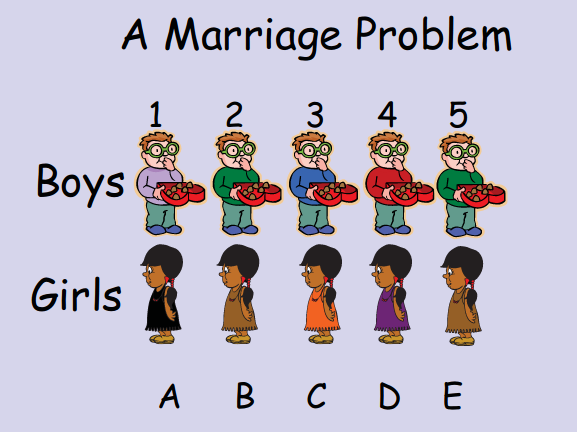
\includegraphics[width=.5\textwidth]{../img/marriage1}\\
    Which boy should marry with which girl?
  \end{center}

\end{frame}

\begin{frame}{The Stable Marriage Problem}{Each boy and girl has a preference list}

  \begin{center}
    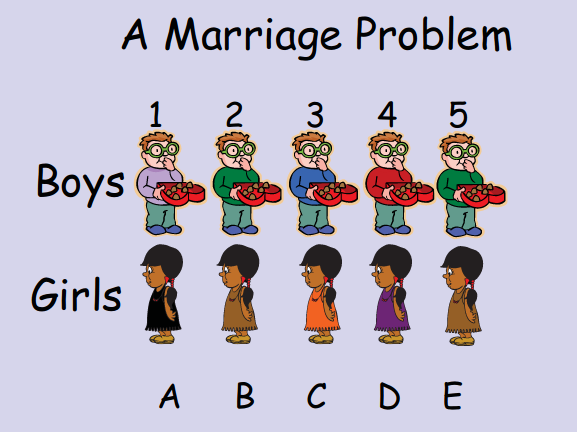
\includegraphics[width=.4\textwidth]{../img/marriage1}
    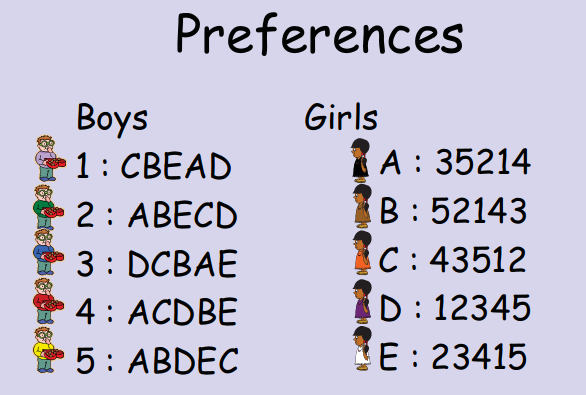
\includegraphics[width=.45\textwidth]{../img/marriage2}
  \end{center}

  Which algorithm do you use to match them?
\end{frame}

\begin{frame}{The "Boy-greedy" algorithm}
  \structure{Boy-greedy algorithm}: Each boy, in order, marries to favorite girl:
  \begin{center}
    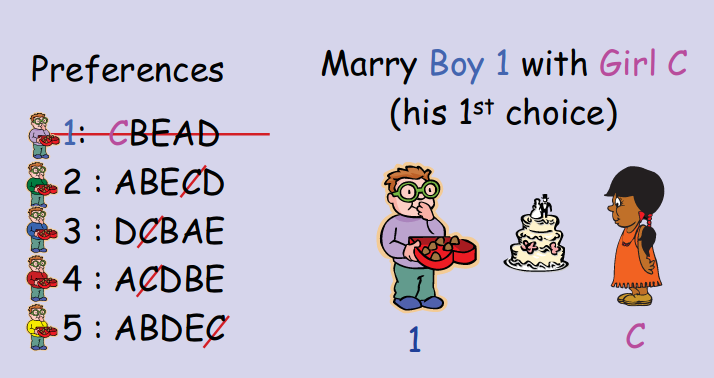
\includegraphics[width=.7\textwidth]{../img/marriage3}
  \end{center}
\end{frame}

\begin{frame}{The "Boy-greedy" Algorithm}

  \structure{Boy-greedy algorithm}: Each boy, in order, marries to favorite girl:
  \begin{center}
    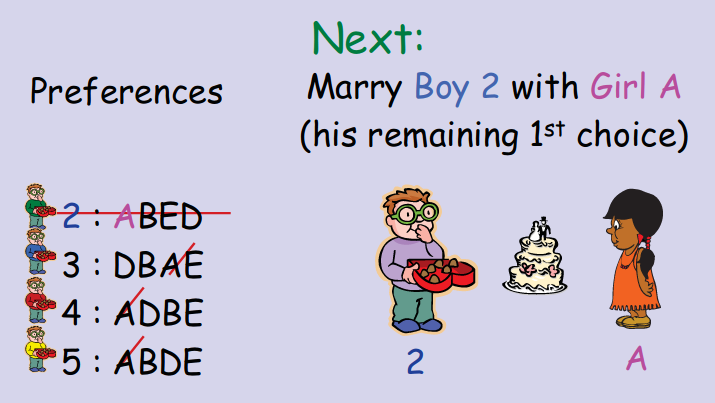
\includegraphics[width=.7\textwidth]{../img/marriage4}
  \end{center}
\end{frame}

\begin{frame}{The "Boy-greedy" Algorithm}{Final Pairings}

  \begin{center}
    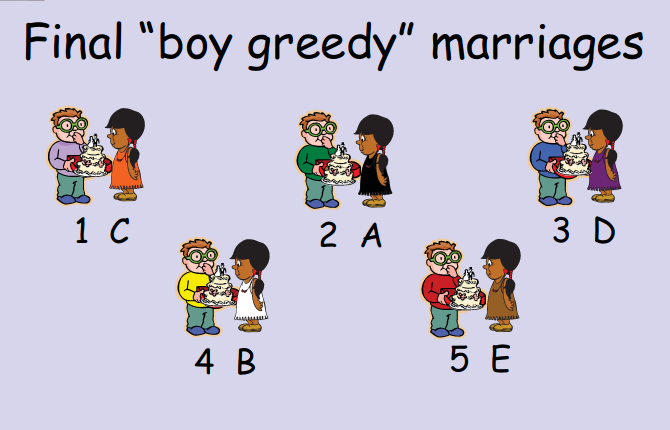
\includegraphics[width=.7\textwidth]{../img/marriage5}
  \end{center}
\end{frame}

\begin{frame}{The "Boy-greedy" Algorithm}{Rogue Couples}
  \begin{center}
    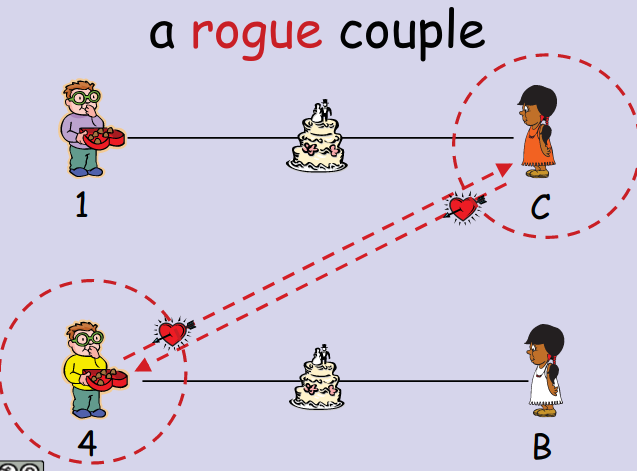
\includegraphics[width=.41\textwidth]{../img/marriage7}
    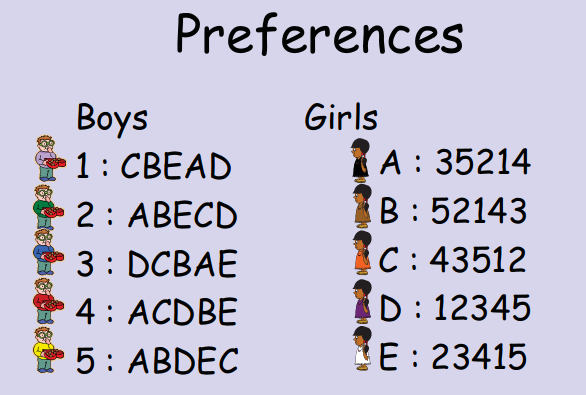
\includegraphics[width=.45\textwidth]{../img/marriage2}
  \end{center}

  \alert{Girl C} likes \structure{Boy 4} better than \structure{Boy 1}. \structure{Boy 4} likes \alert{Girl C} better than \alert{Girl B}.

  Can we find a pairing without rogue couples?
\end{frame}


\begin{frame}{A stable matching}{Using a Girl Greedy algorithm}
  \begin{center}
    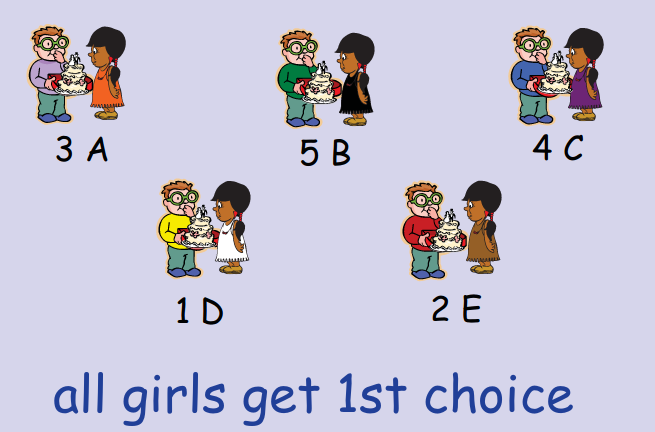
\includegraphics[width=.45\textwidth]{../img/marriage8}
    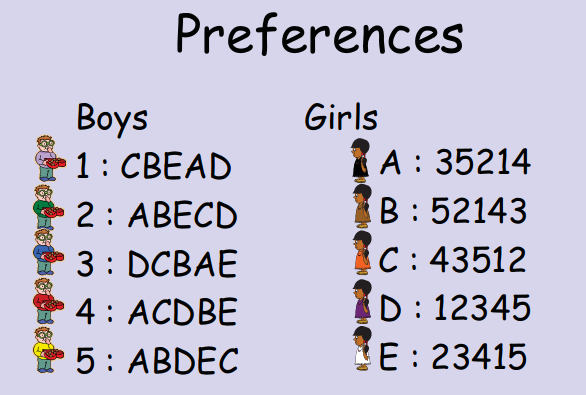
\includegraphics[width=.45\textwidth]{../img/marriage2}
  \end{center}
\end{frame}

\begin{frame}
  \frametitle{Why is the Stable Marriage Problem Important?}

  {\larger
    \begin{itemize}
    \item School Admissions in the US
    \begin{itemize}
      \item Matching school preference and student preference
    \end{itemize}\bigskip


    \item Server/Client Request Matching
    \begin{itemize}
      \item In large webpages, multiple HTTP servers serve the same page for multiple clients;
      \item Servers are matched to clients by geolocation, etc;
    \end{itemize}\bigskip

    \item Etc...
    \end{itemize}
  }
\end{frame}

\subsection{``Mating Ritual'' Algorithm}

\begin{frame}{The ``Mating Ritual'' Algorithm}

    Let us describe an algorithm to {\bf always} find a
    stable matching:\bigskip

    \begin{itemize}
      \item {States}:
      \begin{itemize}
        \item Each boy is proposing to some girl.
        \item Each girl has a list of proposers.
      \end{itemize}
      \item {\bf Start State}: Every boy is proposing to their favorite girl.
    \end{itemize}

    Algorithm:
    \begin{enumerate}
      \item If all girls have $\leq 1$ proposers in their list, they are paired and the algorithm ends;
      \item Any girl with $> 1$ proposers in their list reject all except their favorite proposer;
      \item If a boy is rejected, they propose to the next girl in their list;
      \item Return to (1).
    \end{enumerate}
\end{frame}

\begin{frame}{The Mating Ritual Algorithm}{Example}

  \begin{columns}
    \column{0.45\textwidth}
    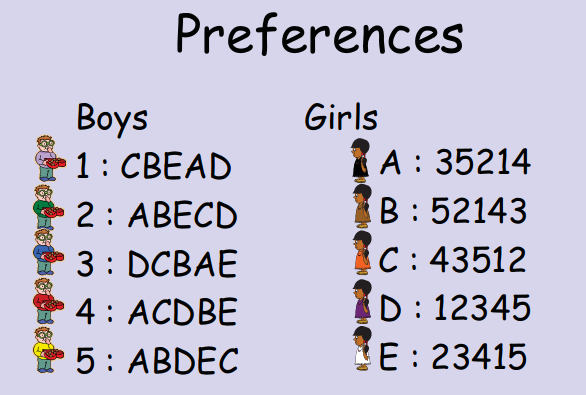
\includegraphics[width=1\textwidth]{../img/marriage2}
    \column{0.55\textwidth}
    {\large
      \begin{itemize}
      \item {\bf iter 1}: No rejections. Proposals:
        \begin{itemize}
        \item A: 2, 4, 5
        \item B:
        \item C: 1
        \item D: 3
        \item E:
        \end{itemize}

      \item {\bf iter 2}: A rejects 2 and 4. Proposals:
        \begin{itemize}
        \item A: 5
        \item B: 2
        \item C: 1, 4
        \item D: 3
        \item E:
        \end{itemize}
      \end{itemize}

    }
  \end{columns}
\end{frame}

\begin{frame}{The Mating Ritual Algorithm}{Example}

  \begin{columns}
    \column{0.45\textwidth}
    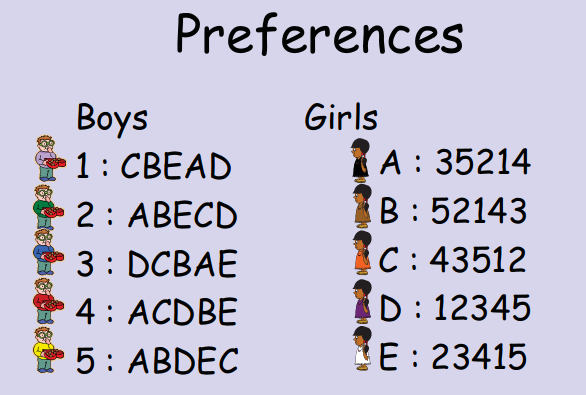
\includegraphics[width=1\textwidth]{../img/marriage2}
    \column{0.55\textwidth}
    {\large
      \begin{itemize}
      \item {\bf iter 3}: C rejects 1. Proposals:
        \begin{itemize}
        \item A: 5
        \item B: 1, 2
        \item C: 4
        \item D: 3
        \item E:
        \end{itemize}

      \item {\bf iter 4}: B rejects 1. Proposals:
        \begin{itemize}
        \item A: 5
        \item B: 2
        \item C: 4
        \item D: 3
        \item E: 1
        \end{itemize}
      \end{itemize}
    }
  \end{columns}
\end{frame}

\begin{frame}{The "Mating Ritual" Algorithm}{Proof of Correctness}

  {\larger
  To proof the correctness of an algorithm, requires that you demonstrate two facts:

    \begin{itemize}
    \item The algorithm stops at some point after the start state;

      \bigskip

    \item The algorithm is correct when it stops;
    \end{itemize}
  }
\end{frame}

\begin{frame}{Proof of Correctness}{The algorithm stops}

  {\larger
    Every day, the \structure{total number} of girls in
    the boy's lists is reduced.

    \bigskip

    \begin{itemize}
      \item Every day, {\bf At least one boy} is rejected by {\bf at least one girl}
      \begin{itemize}
        \item If no boy is rejected, it means that all girls have $\leq 1$ boys in their list
        \item If all girls have $\leq 1$ boys in their list, the algorithm stops;
      \end{itemize}
      \item At some point, every boy's list will have {\bf no girls}:
      \begin{itemize}
        \item A boy with no girls in their list will propose to no one.
        \item If no boys propose, then all girl's lists are empty.
        \item Then the algorithm stops.
      \end{itemize}
    \end{itemize}

    \bigskip

    The total size of "Boy's Lists" is \structure{strictly decreasing}, so the algorithm is guaranteed to stop.
  }
\end{frame}

\begin{frame}
  \frametitle{Proof of Correctness: No rogue couples}

  {\larger

    \begin{itemize}
    \item {\bf Lemma 1}: The rank of a girl's favorite is {\bf weakly
      increasing}\\ Every iteration, the girl rejects a favorite {\bf
      iff} she finds a \structure{better one}.

      \bigskip

    \item {\bf Lemma 2}: The rank of a boy's favorite is {\bf weakly
      decreating}\\ Every iteration, the boy stays with current
      favorite, or is rejected and goes to the next lower one.

    \end{itemize}
  }
\end{frame}

\begin{frame}
  \frametitle{Proof of Correctness: No rogue couples}

  {\larger {\bf Invariant:} If $G_i$ is not on $B_j$ list, she has a
    better curent favorite.

    \bigskip

    \begin{itemize}
      \item At the beginning of the algorithm, $G_i$ is on $B_j$ list;
      \item $G_i$ will reject a boy proposing to her only if a better favorite is also proposing to her;
      \item This implies that a girl's favorite never get worse (lemma 1)
    \end{itemize}
  }
\end{frame}

\begin{frame}
  \frametitle{Proof of Correctness: No rogue couples}

  {\larger

    {\bf Lemma:} When boy $B_i$ is paired, he cannot form a rogue
    couple.

    \bigskip

    {\bf Proof by Cases:}
    \begin{itemize}
    \item {\bf Case 1:} $B_i$ tries to form a rogue couple with
      someone not on his list. However, by \alert{Invariant}, any girl
      not on his list has a better favorite, and no rogue couple is
      possible.

    \item {\bf Case 2:} $B_i$ tries to form a rogue couple with
      someone on his list. However, by \alert{Lemma 2}, $B_i$ always
      propose to the best girl in his list, and no rogue couple is
      possible.
    \end{itemize}

    \bigskip

    {\bf Therefore}, no rogue couple is possible.

  }
\end{frame}

% \begin{frame}
%   \frametitle{Extra Topics}
%
%   {\larger
%
%     Check the class materials for ``Hall's Graphs'', for more
%     information on matching.
%
%   }
%
% \end{frame}
